\chapter{Implementation}




\section{Compression}
\label{section:impl_compression}

To compress the BTF data we used Java. In our case, the main problem of PCA lies in implementation of singular value decomposition (SVD) for a set of images.
To solve this problem, we used a fast linear library \emph{jblas} \cite{jblas} developed by Mikio Braun. 


Compressed data has to be sent to a shader. One of the possible ways to send large arrays of data to the shader, is to send them as textures. 
So, after we perform SVD, we save our resulted matrices $U$, $\Sigma$, $V$ as textures.  Matrices $U$ and $V$ are in interval $[-1;1]$, so we map the data into image domain $[0;1]$.
The following function is used to map the values:  $f(x)=(x+1)/2$.
 Each component of matrix $U$ is stored separately as PNG images. For example, if compressed BTF data has $8$ principal components, then this would result in  $8$ images.
This is done for streaming purposes, so then it would be sent one by one from the server to the client.
As for matrix $V$ it is saved in one texture, as it is not a big of a size.

 Matrix $\Sigma$ is the diagonal matrix, which stores basically eigenvalues for components. So, basically it can be either send as an array to the shader or stored in a texture.
 For convenience purposes, we store it in a texture. The problem is that the values can be bigger than 256, thus not possible to map explicitly to the texture. 
 Some certain encoding is needed to store it in a texture. In our case
 

Also, one practical consideration when using \emph{jblas} is to scale the data for better reconstructing quality in the shader. We found out that tenths of values of $U$ and $V$ matrices are zeros.
So, basically we can scale the data by multiplying it with $10$ and at the same time matrix $\Sigma$ by $0.1$. This way the reconstruced resulted will the same. But, with scaling we improves precision of the data when we map it.



\section{Rendering}
\label{section:impl_rendering}


The aim of this thesis was to implement efficient BTF-shader for XML3D \cite{xml3d}. XML3D platform was implemented to deploy 3D graphics in web browsers. This technology is based on WebGL and JavaScript.
We also use Xflow \cite{xflow} to combine principal component textures in one texture, which further is needed for BTF-shader. The shader is written in OpenGL Shading Language (GLSL). 
The rendering process of the shader is depicted in figure \ref{fig:shader}.

The compressed BTF data is stored in two textures. One texture $L$ stores principal components, the other $R$ stores PCA weights, which determine how the components have to be summed up.
The other inputs are texture coordinates, eye and light positions. Eye and light positions are transformed to spherical coordinates.
 Then, we lookup the three closest views from the measured BTF data, which are will be needed for interpolation purpose.
 This lookup process is fairly simple as we have a static array in the shader, which stores sample intervals of the measured BTF data.

 




\begin{figure}[h]
 \centering
 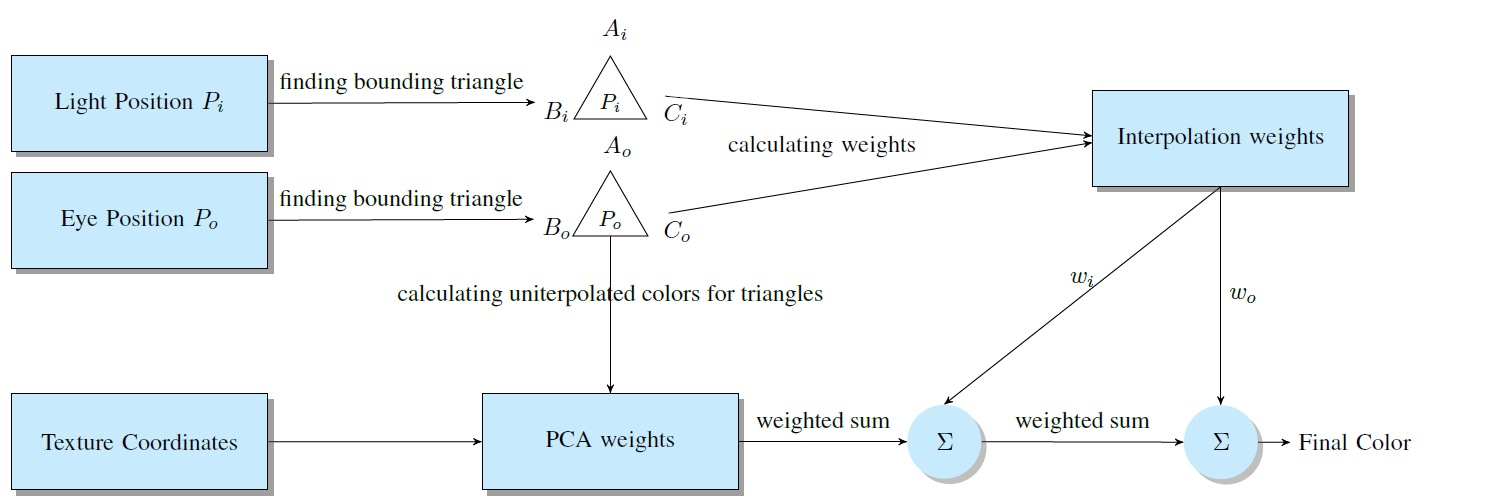
\includegraphics[width=1.0\textwidth]{figures/shader}
 \caption[Shader Design] {
 	{\bf Shader Design }

 }
 \label{fig:shader}
\end{figure}


\section{Streaming}
\label{section:impl_streaming}


Xflow is a part of XML3D implementation, which allows to process the data on flow, i.e. in runtime.
At start, on a client side we create array \emph{texData} of RGB colors, which further will be fulfilled with newly arrived principal components. 
As it was described in chapter \ref{section:streaming}, we stream principal components one by one. Each component $C_{i}$ arrives as a PNG image. 
Then, on a client side we read PNG image using PNG decoder written in JavaScript by Arian Stolwijk \cite{pngreader}.
PNG images are decoded to pure array of RGB colors. This new data of component $C_{i}$ is then placed to its place in \emph{texData}  array. Finally, using Xflow we create from \emph{texData}  array a texture with which we update our BTF-shader.


\begin{figure}[h]
 \centering
 \includegraphics[width=1.0\textwidth]{figures/streampreview}
 \caption[Example of Progressive Streaming ] {
 	{\bf Example of Progressive Streaming}

	\textbf{From left to right}: \emph{1}, \emph{2}, \emph{4}, \emph{6}, \emph{7}  components rendered at the same time.
	
	\textbf{Note}: \emph{8th} component is average grey value, which sends at first place.
	}
 \label{fig:streamPreview}
\end{figure}
\label{chapter:implementation}



Consider Figure \ref{fig:streaming} that shows how the streaming works on practice.
We can see that even with first components the resulted texture looks quite decent.
With further components the overall quality of texture improves, e.g. specularities are increasing, small micro-structures become more visible and emphasized.
To make the streaming process a bit entertaining, the client also can see the progress-bar of the streaming progress.
Also, some of the mid-results were skipped in the Figure \ref{fig:streamPreview} for the sake of simplicity.
